\documentclass[12pt,a4paper]{article}
\usepackage[T1]{fontenc}
\usepackage[utf8]{inputenc}
\usepackage[magyar]{babel}
\usepackage{geometry}
\usepackage{parskip}
\usepackage{booktabs}
\usepackage{array}
\usepackage{longtable}
\usepackage{graphicx}
\usepackage{listings}
\usepackage{needspace} % megakadályozza, hogy egy rövid lstlisting két oldal közt törjön
\usepackage{xcolor}
\usepackage{hyperref}
\usepackage{titlesec}
\usepackage{fancyhdr}
\usepackage{setspace}
\usepackage{amsmath}
\usepackage{amssymb}
\usepackage{caption}
\usepackage{float}
\usepackage{enumitem}
\usepackage[numbers,sort&compress]{natbib}
\usepackage{tikz}
\usetikzlibrary{arrows.meta,positioning,calc}
\usepackage{pgfplots}
\pgfplotsset{compat=1.18}

% A \texttt (monospace) alapértelmezésben nem tör sort kötőjelnél (pl.
% "chirpstack-gateway-bridge"), mert a tt-betűtípus \hyphenchar-ja -1.
% Ez táblázatcellákban (p{} oszlop) a szöveg kilógásához vezet -- az alábbi
% sor minden \ttfamily-váltásnál visszaállítja a kötőjelnél törést.
\let\origttfamily\ttfamily
\renewcommand{\ttfamily}{\origttfamily\hyphenchar\font=`\-\relax}

\geometry{margin=2.5cm}
\setstretch{1.3}

\definecolor{codegray}{rgb}{0.95,0.95,0.95}
\definecolor{keywordcolor}{rgb}{0,0,0.6}
\lstset{
  backgroundcolor=\color{codegray},
  basicstyle=\ttfamily\small,
  keywordstyle=\color{keywordcolor}\bfseries,
  breaklines=true,
  frame=single,
  captionpos=b,
  numbers=left,
  numberstyle=\tiny,
  stepnumber=1,
  tabsize=4,
}

\pagestyle{fancy}
\fancyhf{}
\rhead{Diplomamunka 2026/2027}
\lhead{Nagy Szabolcs}
\rfoot{\thepage}

\hypersetup{
  colorlinks=true,
  linkcolor=black,
  urlcolor=blue,
  citecolor=black
}

% -----------------------------------------------------------------------
\begin{document}
% -----------------------------------------------------------------------

\begin{titlepage}
    \centering
    \vspace*{1cm}
    {\large Óbudai Egyetem\\
    Neumann János Informatikai Kar\\
    Kiberfizikai Rendszerek Intézet}

    \vspace{3cm}
    {\LARGE\bfseries A LoRaWAN hálózatok biztonsági\\[0.3em]
    elemzése és sebezhetőségei\\[0.3em]
    tesztkörnyezetben}

    \vspace{0.5em}
    {\large\itshape Security Analysis and Vulnerabilities\\
    of LoRaWAN Networks in a Testbed Environment}

    \vspace{3cm}
    {\large\bfseries Diplomamunka}

    \vspace{2cm}
    \begin{tabular}{rl}
        \textbf{Szerző:}       & Nagy Szabolcs \\
        \textbf{Neptun-kód:}   & CGZNU9 \\
        \textbf{Témavezető:}   & Balázsné Dr.\ Kail Eszter \\
        \textbf{Konzulens:}    & Bringye Zsolt \\
        \textbf{Intézet:}      & Kiberfizikai Rendszerek Intézet \\
        \textbf{Képzés:}       & Kiberbiztonsági mérnöki MSc \\
    \end{tabular}

    \vfill
    {\large Budapest, 2026/2027. tanév}
\end{titlepage}

% -----------------------------------------------------------------------
\tableofcontents
\newpage

% -----------------------------------------------------------------------
\section*{Összefoglaló}
\addcontentsline{toc}{section}{Összefoglaló}
% -----------------------------------------------------------------------

A LoRaWAN (Long Range Wide Area Network) protokoll az IoT-kommunikáció egyik
legelterjedtebb megoldása kritikus infrastruktúrákban, okosvárosi rendszerekben
és ipari környezetekben. A protokoll AES-128 alapú titkosítást és
üzenethitelesítést alkalmaz, azonban a fizikai eszközök és a valós telepítések
biztonsága számos ponton sebezhetőséget mutat.

Jelen dolgozatban bemutatjuk egy Óbudai Egyetemen felépített LoRaWAN
tesztkörnyezet segítségével elvégzett biztonsági vizsgálat eredményeit.
Négy különálló támadási forgatókönyvet valósítottunk meg és demonstráltunk:
(1)~passzív rádiós lehallgatás SDR eszközzel, (2)~SPI-busz lecsapolás
logikai analizátorral az MCU--rádióchip interfészen, (3)~AppKey szótáras és
kimerítő keresés a Join~Request MIC alapján, valamint (4)~firmware-binárisból
automatizált hitelesítőadat-kinyerés és álcázott csomópont generálása.

A tesztkörnyezetben vizsgált LoRaWAN csomópont esetén az SPI-busz tap teljes
plaintext hozzáférést adott a LoRaWAN keretekhez, a passzív sniffing pedig az
összes Join~Request metaadatát (AppEUI, DevEUI, DevNonce, MIC) feltárta
hálózati hozzáférés nélkül. Az AppKey brute-force gyenge kulcsok esetén
milliszekundumokon belül sikeres volt. Végül bemutattuk, hogy a firmware-szintű
titkosítás bekapcsolása hatékonyan véd a közvetlen flash-dump alapú
kulcskinyeréssel szemben.

Az eredmények rámutatnak arra, hogy az alkalmazott kriptográfiai védelem
önmagában nem elégséges, és a fizikai biztonsági intézkedések, az erős
kulcsmenedzsment, valamint a hardened firmware-konfiguráció együttes alkalmazása
szükséges a valós fenyegetési modell kezeléséhez.

\bigskip
\noindent\textbf{Kulcsszavak:} LoRaWAN, IoT-biztonság, SPI-busz tap,
SDR sniffing, AppKey, brute-force, firmware-elemzés, tesztkörnyezet, embedded
security

\bigskip
\noindent\textbf{Abstract.} This paper presents the results of a security
evaluation conducted on a LoRaWAN testbed built at Óbuda University.
We demonstrate four attack scenarios against a commercial LoRaWAN end device:
passive radio sniffing via SDR, physical SPI bus tap between the MCU and radio
chip, AppKey recovery through dictionary and exhaustive brute-force of the
Join Request MIC, and automated credential extraction from a firmware binary
with rogue-node generation. Our findings show that the AES-128 cryptographic
protection specified by the LoRaWAN standard is insufficient when physical
access or weak key management is present. We also evaluate the effectiveness
of firmware-level flash encryption as a mitigation.

\bigskip
\noindent\textbf{Keywords:} LoRaWAN, IoT security, SPI bus tap, SDR sniffing,
AppKey, brute-force, firmware analysis, testbed, embedded security

\newpage

% -----------------------------------------------------------------------
\section{Bevezetés}
% -----------------------------------------------------------------------

Az IoT (Internet of Things) eszközök robbanásszerű elterjedése az elmúlt
évtizedben számos új biztonsági kihívást hozott magával. A LoRaWAN protokoll
a kis fogyasztású, nagy hatótávolságú vezeték nélküli kommunikáció területén
kiemelkedő szerepet tölt be: okos vízórák, gázdetektorok, ipari szenzorok
és okosvárosi infrastruktúra-elemek tömegei kommunikálnak ezen a protokollon.

A LoRaWAN biztonsági modellje AES-128 alapú kriptográfiai védelmet nyújt mind
az alkalmazásrétegen (AppSKey), mind a hálózati rétegen (NwkSKey). A Join
mechanizmus ezenkívül friss munkamenetkulcsokat állít elő minden csatlakozásnál.
Ennek ellenére a valós biztonsági kép összetettebb: a kulcsanyag a végpontok
flash memóriájában tárolódik, az eszközök fizikailag hozzáférhetők, és az
iparági tapasztalatok szerint a gyártók és integrátorok rendszeresen alkalmaznak
gyenge vagy alapértelmezett kulcsokat.

Jelen diplomamunka az ÓE-NIK Kiberfizikai Rendszerek Intézetén felépített
LoRaWAN tesztkörnyezet segítségével elvégzett biztonsági vizsgálat eredményeit
mutatja be, módszertanában az iparági biztonsági felmérések
gyakorlatához igazodva~\cite{bertran2018}.

A dolgozat struktúrája a következő: a 2.\ fejezet a LoRaWAN protokollt és
biztonsági modelljét ismerteti; a 3.\ fejezet a tesztkörnyezet felépítését
mutatja be; a 4--7.\ fejezetek a négy demonstrált támadási forgatókönyvet
tárgyalják; a 8.\ fejezet a védelmi mechanizmusokat értékeli; a 9.\ fejezet
összefoglalja az eredményeket és jövőbeli kutatási irányokat javasol.

% -----------------------------------------------------------------------
\section{A LoRaWAN protokoll és biztonsági modellje}
% -----------------------------------------------------------------------

\subsection{Protokoll-architektúra}

A LoRaWAN egy csillag-topológiájú, aszimmetrikus kommunikációs protokoll,
amelynek négy fő komponense van: végpont eszközök (end devices), átjárók
(gateways), hálózati szerver (network server) és alkalmazásszerver
(application server). Az átjárók LoRa modulált csomagokat vesznek és
továbbítanak IP-alapú backhaulon a hálózati szerverre.

A LoRa fizikai réteg Chirp Spread Spectrum (CSS) modulációt alkalmaz,
az SF (Spreading Factor) 7-től 12-ig változhat: nagyobb SF nagyobb hatótávolságot,
de alacsonyabb adatátviteli sebességet jelent. Az EU868-as sávban a protokoll
meghatározott csatornakészleten (868,1~MHz, 868,3~MHz, 868,5~MHz stb.)
működik.

\subsection{Biztonsági modell és kulcsarchitektúra}

A LoRaWAN~1.0.x specifikáció szerint~\cite{lorawan104} minden eszköz rendelkezik:
\begin{itemize}
    \item \textbf{AppKey} (128 bites) -- a gyökér szimmetrikus kulcs, amelyből a
    munkamenetkulcsok levezethetők,
    \item \textbf{AppEUI} és \textbf{DevEUI} -- 64 bites azonosítók,
    \item \textbf{DevAddr} -- 32 bites hálózati cím, amelyet a szerver oszt ki
    a Join eljárás során.
\end{itemize}

Az OTAA (Over-the-Air Activation) csatlakozási eljárásban az eszköz Join~Request
üzenetet küld, amelyet a szerver Join~Accept üzenettel nyugtáz. A munkamenetkulcsok
levezetése:
\begin{align}
    \text{NwkSKey} &= \text{AES-128}(\text{AppKey},\ 0\text{x}01
    \mathbin\| \text{AppNonce} \mathbin\| \text{NetID} \mathbin\| \text{DevNonce}
    \mathbin\| \text{pad}_{16}) \\
    \text{AppSKey} &= \text{AES-128}(\text{AppKey},\ 0\text{x}02
    \mathbin\| \text{AppNonce} \mathbin\| \text{NetID} \mathbin\| \text{DevNonce}
    \mathbin\| \text{pad}_{16})
\end{align}

Az adatkeretek payloadja AppSKey-jel titkosított (AES-128-CTR), integritásukat
NwkSKey-jel számolt MIC védi.

\begin{figure}[H]
\centering
\resizebox{0.92\textwidth}{!}{%
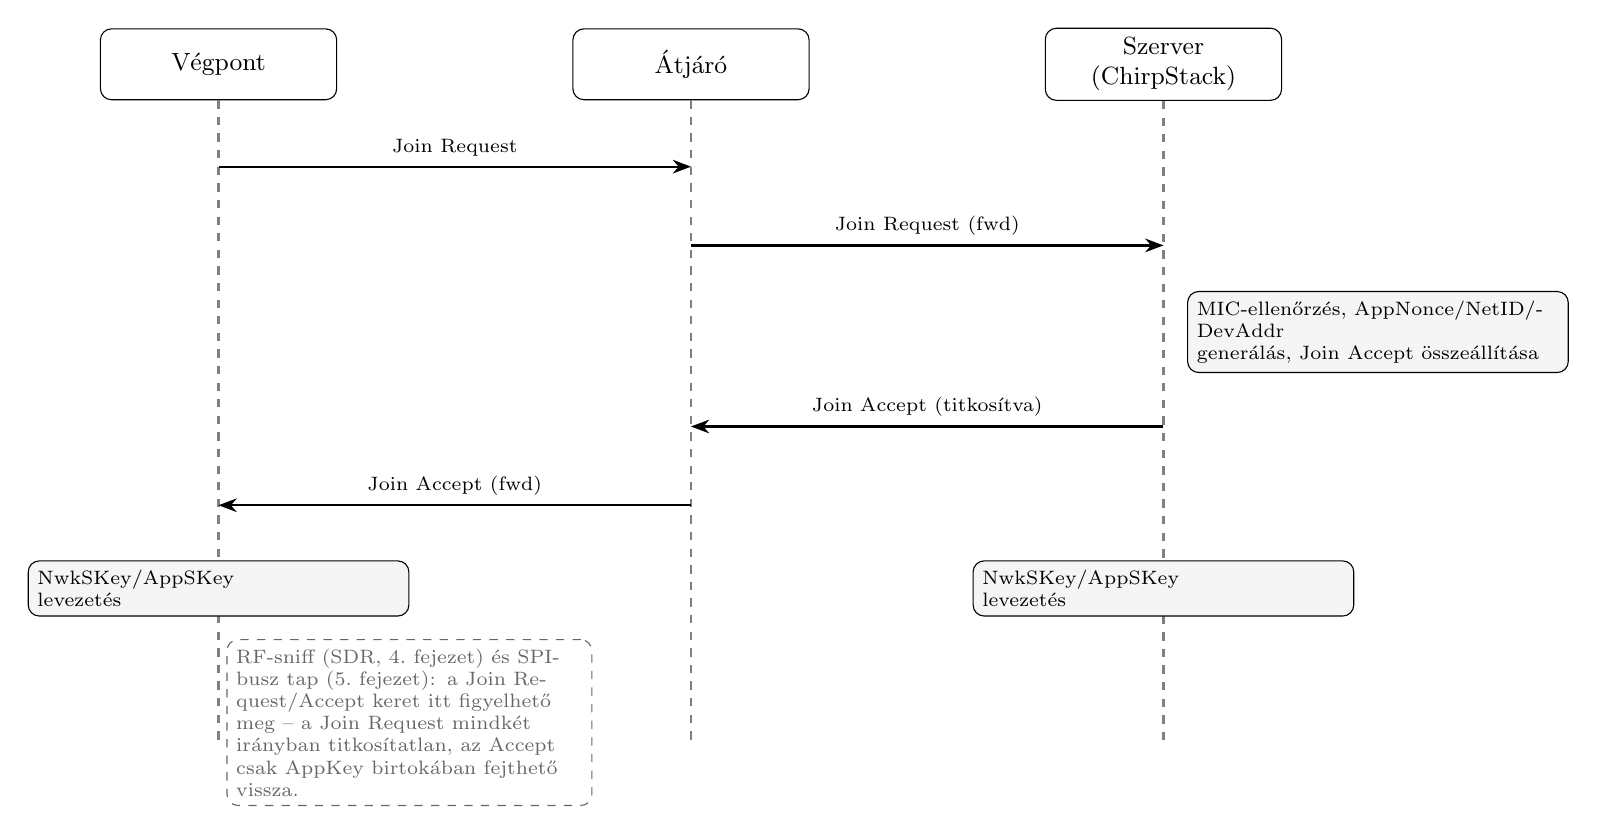
\begin{tikzpicture}[
  actor/.style={draw, rounded corners, align=center, minimum width=3.0cm, minimum height=0.9cm, font=\small},
  lifeline/.style={dashed, thick, gray},
  msg/.style={-{Stealth}, thick},
  note/.style={draw, rounded corners, align=left, font=\scriptsize, fill=gray!8, text width=4.6cm},
  atk/.style={draw, dashed, rounded corners, align=left, font=\scriptsize, color=black!60, text width=4.4cm}
]
\node[actor] (node) at (0,0) {Végpont};
\node[actor] (gw) at (6,0) {Átjáró};
\node[actor] (srv) at (12,0) {Szerver\\(ChirpStack)};
\draw[lifeline] (node.south) -- ++(0,-8.2);
\draw[lifeline] (gw.south) -- ++(0,-8.2);
\draw[lifeline] (srv.south) -- ++(0,-8.2);
\draw[msg] (0,-1.3) -- node[above, font=\scriptsize]{Join Request} (6,-1.3);
\draw[msg] (6,-2.3) -- node[above, font=\scriptsize]{Join Request (fwd)} (12,-2.3);
\node[note, anchor=west] at (12.3,-3.4) {MIC-ellenőrzés, AppNonce/NetID/DevAddr\\generálás, Join Accept összeállítása};
\draw[msg] (12,-4.6) -- node[above, font=\scriptsize]{Join Accept (titkosítva)} (6,-4.6);
\draw[msg] (6,-5.6) -- node[above, font=\scriptsize]{Join Accept (fwd)} (0,-5.6);
\node[note, anchor=north] at (0,-6.3) {NwkSKey/AppSKey\\levezetés};
\node[note, anchor=north] at (12,-6.3) {NwkSKey/AppSKey\\levezetés};
\node[atk, anchor=north west] at (0.1,-7.3) {RF-sniff (SDR, 4.\ fejezet) és SPI-busz tap (5.\ fejezet): a Join Request/Accept keret itt figyelhető meg -- a Join Request mindkét irányban titkosítatlan, az Accept csak AppKey birtokában fejthető vissza.};
\end{tikzpicture}}
\caption{Az OTAA Join-folyamat üzenetváltása és a két passzív megfigyelési pont
(Végpont oldali SPI-tap, illetve a rádiós link SDR-sniffelése).}
\end{figure}

\subsection{Ismert sérülékenységek a szakirodalomban}

A LoRaWAN biztonsági modelljének gyengeségeit több független kutatás is
vizsgálta~\cite{yang2018, aras2017, butun2018, Loukil2018, Noura2020}. Az alábbiakban a dolgozat
szempontjából releváns, ismétlődően felmerülő problémákat tekintjük át; a
4--7.\ fejezetben bemutatjuk, melyik ismert probléma az, amit a saját
tesztkörnyezetben is sikerült demonstrálni, és melyik marad ezen dolgozat
keretein kívül eső, pusztán elméleti kockázat.

\paragraph{Replay-támadás (DevNonce-újrafelhasználás).} A LoRaWAN~1.0.x
szabványban a Join~Request DevNonce mezője mindössze 16 bites, véletlenszerű
érték~\cite{yang2018}. A specifikáció előírja, hogy a Join Server tartsa
nyilván az adott eszköztől már látott DevNonce-értékeket, és utasítsa el az
ismétlődőket -- azonban ez az implementációk minőségén múlik, és több
kereskedelmi hálózati szerver-megvalósításban hiányosan volt implementálva
vagy megkerülhető volt~\cite{aras2017}. Ha egy korábban rögzített, érvényes
Join~Request visszajátszható, az minden esetben új munkamenetkulcs-párt
(NwkSKey/AppSKey) vált ki a szerver oldalán -- ez önmagában nem ad hozzáférést
a kulcsokhoz, de szolgáltatás-megtagadást (a legitim eszköz munkamenete
érvénytelenítődik) vagy a hálózati napló megzavarását teheti lehetővé. A
Join-eljárás formális biztonsági elemzése és konkrét, kombinált
visszajátszás-alapú támadási forgatókönyvek is megerősítik, hogy ez a
felület a gyakorlatban is kihasználható, nemcsak elméletben~\cite{Tomasin2017,
Le2021, Wesemeyer2020, Eldefrawy2019}.

\paragraph{Bit-flipping és a csonkított MIC.} A payload titkosítása AES-128
CTR (counter) módban történik, ami -- minden stream cipherhez hasonlóan --
malleábilis: a titkosított szöveg egy bitjének megváltoztatása a
visszafejtett plaintext ugyanazon bitjét változtatja meg, anélkül, hogy a
titkosítás önmagában ezt jelezné~\cite{yang2018}. Ismert (vagy kitalálható)
plaintext-struktúra esetén (pl.\ fix formátumú szenzoradat-keretek) ez
célzott payload-manipulációt tesz lehetővé. Az integritásvédelem a
128 bites AES-CMAC-ból számolt, de a keretben csak 4 bájtra (32 bitre)
csonkított MIC -- egy vak, találgatáson alapuló hamisítás sikerességi esélye
emiatt $2^{-32}$ próbánkénti keretre adódik, ami lényegesen alacsonyabb
biztonsági margót jelent, mint egy teljes 128 bites MAC-nál, és a
szakirodalomban rendszeresen felmerülő kritikai pont~\cite{butun2018}.

\paragraph{ACK spoofing.} Megbízhatósági (confirmed) uplink keretek esetén az
eszköz egy hálózati oldali ACK-ra vár nyugtázásként. Mivel az ACK a
letöltési (downlink) ablakban érkezik, egy támadó -- aki a gateway és a
hálózati szerver közti csatornát, vagy magát az RF-linket kontrollálja --
hamis ACK-ot injektálhat, ami azt a látszatot kelti az eszköznek, hogy az
üzenet célba ért, miközben az valójában sosem jutott el a
szerverig~\cite{aras2017}. Ez különösen kritikus, ha az alkalmazás logika a
sikeres kézbesítést biztonsági- vagy vészjelzés nyugtázásaként kezeli --
hasonló ember-a-középen (MITM) forgatókönyveket valós tesztkörnyezetben is
demonstráltak~\cite{Thomas2020, Pospisil2021}.

\paragraph{RF jamming és szolgáltatás-megtagadás.} Az EU868 sávban a
LoRaWAN egy rögzített, kis méretű csatornakészleten (jellemzően 8 alap
csatorna, 125~kHz sávszélesség) működik, szigorú duty cycle-korláttal (~1\%
csatornánként)~\cite{butun2018}. A fix csatornakészlet és a korlátozott
adóteljesítmény miatt egy célzott zavaró jel viszonylag olcsón és
energiahatékonyan tud teljes területi lefedettségű szolgáltatás-megtagadást
okozni -- ezzel szemben a szabvány önmagában nem nyújt védelmet
(frekvencia-ugratás vagy spread-spectrum ellenállás korlátozott a rögzített
csatornaterv miatt). Kereskedelmi hardverrel épített szelektív és reaktív
zavaró eszközökkel ezt a sebezhetőséget valós méréssel is igazolták, és a
fizikai rétegbeli LoRaWAN-támadások szisztematikus áttekintése is a
jamminget sorolja a legkönnyebben kivitelezhető fenyegetések
közé~\cite{ArasJam2017, Perkovi2021, Ruotsalainen2022}.

\paragraph{ABP-aktiváció és a forward secrecy hiánya.} Az ABP (Activation
By Personalization) aktivációs módnál nincs Join-folyamat: a DevAddr és a
két munkamenetkulcs (NwkSKey, AppSKey) statikusan, gyártáskor kerül az
eszközbe, és soha nem cserélődik, amíg valaki manuálisan le nem cseréli
őket~\cite{yang2018}. Ez egyrészt megszünteti a DevNonce-alapú
replay-védelmet (nincs újra-Join, amit védeni kellene), másrészt közvetlenül
összefügg a CTR-mód keystream-újrafelhasználási kockázatával: ha egy eszköz
keretszámlálója (FCnt) bármilyen okból (reset, firmware-flash, óraátállás)
egy már korábban használt értékre áll vissza, a payload-titkosítás
keystreamje ismétlődik, ami -- ismert plaintext birtokában -- a titkosítás
teljes megkerülését teszi lehetővé.

\paragraph{Fizikai rétegbeli ujjlenyomat-vétel, mint detekciós ellenintézkedés.}
A fenti támadások jelentős része (replay, ACK spoofing, rogue node) közös
tulajdonsága, hogy a hamis keret a protokoll szintjén hitelesnek tűnhet, ha a
támadó ismeri (vagy visszajátssza) a szükséges azonosítókat. Robyns és
szerzőtársai megmutatták, hogy az adók rádiófrekvenciás
lenyomata (a jelalak apró, hardverfüggő torzításai) felügyelt és zero-shot
tanulási módszerekkel megkülönböztethető, így elméletileg lehetőség nyílik
egy klónozott vagy rogue eszköz protokoll-szinten észrevehetetlen
kommunikációjának fizikai rétegen történő felismerésére~\cite{robyns2017}. Ez
a dolgozat 7.\ fejezetében bemutatott álcázott csomóponttal szemben releváns,
de jelenleg nem megvalósított védelmi irány. Újabb kutatások azt is
megmutatták, hogy ez a fizikai ujjlenyomat-vétel maga is támadható:
ellenséges (adversarial) perturbációval megtévesztő vagy álcázó jelalak
állítható elő mélytanulás-alapú detektorok ellen, ami a védelmi irány
hosszú távú megbízhatóságát önmagában is megkérdőjelezi~\cite{Sagduyu2023,
Sagduyu2025}.

A LoRaWAN~1.1-es specifikáció~\cite{lorawan11} a fenti problémák egy részét
kezeli: a DevNonce-t 16 bites véletlen értékről monoton növekvő számlálóra
cseréli (kezelve a replay-kockázatot resetelő eszközöknél is), bevezeti a
JoinEUI-t (az AppEUI kiterjesztése/átnevezése), és a NwkSKey-t három
különálló kulcsra bontja (SNwkSIntKey, FNwkSIntKey, NwkSEncKey), csökkentve
egy esetleges kulcsszivárgás hatókörét. A piacon -- így a jelen
tesztkörnyezetben vizsgált eszköz esetén is -- azonban túlnyomórészt még
1.0.x eszközök vannak forgalomban, ezért a dolgozat fókusza is az 1.0.x
biztonsági modellen marad.

% -----------------------------------------------------------------------
\section{A tesztkörnyezet felépítése}
% -----------------------------------------------------------------------

\subsection{Hardver-komponensek}

A tesztkörnyezet az alábbi komponensekre épül:

\begin{table}[H]
\centering
\caption{A tesztkörnyezet hardver-elemei}
\begin{tabular}{lll}
\toprule
Komponens & Eszköz & Szerepkör \\
\midrule
Végpont csomópont & kereskedelmi LoRaWAN node & OTAA kliens \\
Átjáró & kereskedelmi LoRaWAN GW & LoRaWAN GW \\
Hálózati szerver & ChirpStack v4 & szoftver szerveren \\
Passzív sniffer & SDR vevő + antenna & rádiós megfigyelés \\
Logikai analizátor & logikai analizátor & SPI-busz tap \\
\bottomrule
\end{tabular}
\end{table}

A vizsgált LoRaWAN csomópont egy integrált MCU + rádióchip megoldáson alapul.
Az MCU és a rádióchip közötti SPI-busz pinjai hozzáférhetők a PCB-n,
ami lehetővé teszi a fizikai lehallgatást.
Alapértelmezetten a firmware-szintű titkosítás és a biztonságos indítás
nincsenek bekapcsolva.

\subsection{Szoftver-stack}

A végpontokon nyílt forráskódú LoRaWAN firmware stack fut.
A hálózati szerver ChirpStack~v4.19.0~\cite{chirpstack}, konténerizált
(docker-compose) architektúrában futtatva:

\begin{table}[H]
\centering
\caption{A hálózati szerver oldal szoftver-komponensei}
\small
\begin{tabular}{@{}p{3.1cm}p{4.3cm}p{6.6cm}@{}}
\toprule
Szolgáltatás & Image & Szerepkör \\
\midrule
\texttt{chirpstack} & \texttt{chirpstack/chirpstack:4} & LoRaWAN network server (API+UI) \\
\texttt{chirpstack-gateway-bridge} & \texttt{chirpstack/chirpstack-gateway-bridge:4} & Gateway$\leftrightarrow$NS packet forwarder híd \\
\texttt{chirpstack-rest-api} & \texttt{chirpstack/chirpstack-rest-api:4} & REST/JSON $\leftrightarrow$ gRPC gateway \\
\texttt{postgres} & \texttt{postgres:14-alpine} & ChirpStack adatbázis \\
\texttt{redis} & \texttt{redis:7-alpine} & ChirpStack cache/session \\
\texttt{mosquitto} & \texttt{eclipse-mosquitto:2} & MQTT broker (integráció, uplink-publikálás) \\
\bottomrule
\end{tabular}
\end{table}

A szerverhez távoli hozzáférés egy dedikált, nem-admin operációs fiókkal
történik, amely kizárólag a projektmappára és a Docker-parancsok
futtatására jogosult -- ez tudatos, minimál jogosultságú
hozzáférés-tervezési döntés, nem az alapértelmezett adminisztrátori profil
használata.

A passzív snifferhez GNU~Radio alapú pipeline-t és LoRa dekódoló modult
alkalmazunk.

\subsection{A tesztkörnyezet elrendezése}

A laboratóriumi elrendezés biztosítja, hogy az összes támadási forgatókönyv
kontrollált és megismételhető körülmények között hajtható végre. A végpontok
EU868-as sávon, SF7, BW125~kHz, CR4/5 paraméterekkel kommunikálnak.

\begin{figure}[H]
\centering
\resizebox{\textwidth}{!}{%
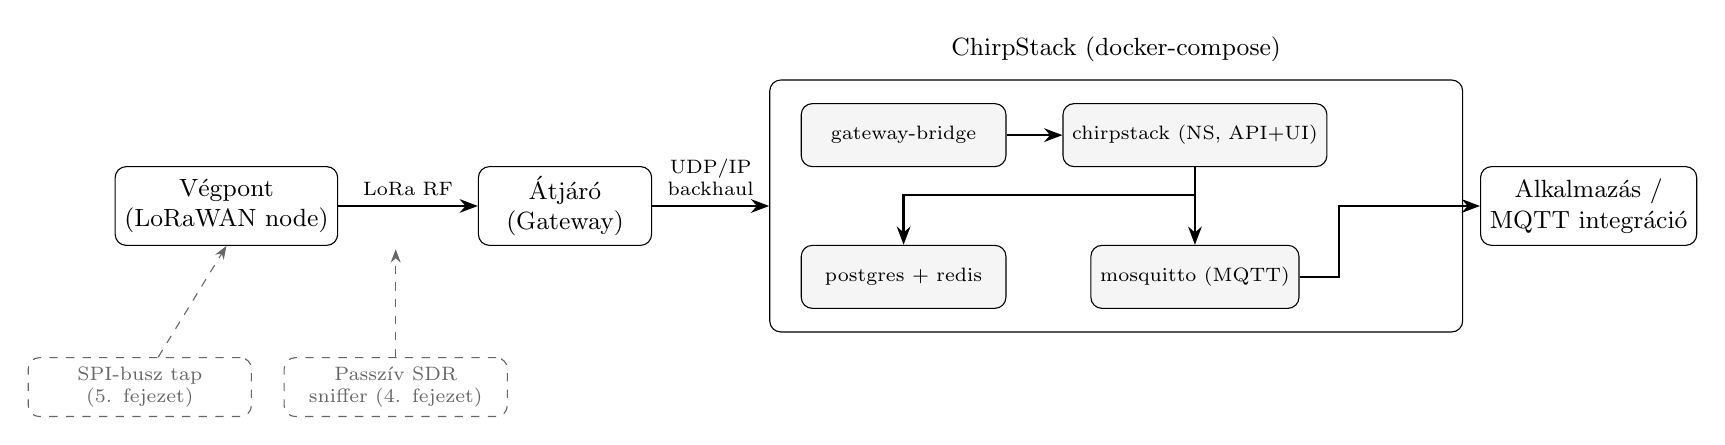
\begin{tikzpicture}[
  box/.style={draw, rounded corners, align=center, minimum width=2.2cm, minimum height=1cm, font=\small},
  svc/.style={draw, rounded corners, align=center, minimum width=2.6cm, minimum height=0.8cm, font=\scriptsize, fill=gray!8},
  srvbox/.style={draw, rounded corners, minimum width=8.8cm, minimum height=3.2cm},
  arr/.style={-{Stealth}, thick},
  atk/.style={draw, dashed, rounded corners, font=\scriptsize, align=center, text width=2.6cm, color=black!60},
  atkarr/.style={-{Stealth}, dashed, color=black!60}
]
\node[box] (node) at (0,0) {Végpont\\(LoRaWAN node)};
\node[box] (gw) at (4.3,0) {Átjáró\\(Gateway)};
\node[srvbox] (srv) at (11.3,0) {};
\node[font=\small, anchor=south] at ($(srv.north)+(0,0.1)$) {ChirpStack (docker-compose)};
\node[svc] (bridge) at ($(srv.center)+(-2.7,0.9)$) {gateway-bridge};
\node[svc] (cs) at ($(srv.center)+(1.0,0.9)$) {chirpstack (NS, API+UI)};
\node[svc] (db) at ($(srv.center)+(-2.7,-0.9)$) {postgres + redis};
\node[svc] (mq) at ($(srv.center)+(1.0,-0.9)$) {mosquitto (MQTT)};
\node[box] (app) at (17.3,0) {Alkalmazás /\\MQTT integráció};
\draw[arr] (node) -- node[above, font=\scriptsize]{LoRa RF} (gw);
\draw[arr] (gw) -- node[above, font=\scriptsize, align=center]{UDP/IP\\backhaul} (srv.west);
\draw[arr] (bridge.east) -- (cs.west);
\draw[arr] (cs.south) -- ++(0,-0.35) -| (db.north);
\draw[arr] (cs.south) -- (mq.north);
\draw[arr] (mq.east) -- ++(0.5,0) |- (app.west);
\node[atk] (sdr) at (2.15,-2.3) {Passzív SDR sniffer (4. fejezet)};
\draw[atkarr] (sdr) -- (2.15,-0.55);
\node[atk] (spi) at (-1.1,-2.3) {SPI-busz tap (5. fejezet)};
\draw[atkarr] (spi) -- (node.south);
\end{tikzpicture}}
\caption{A tesztkörnyezet architektúrája: a végponttól a hálózati szerveren át
az alkalmazásig, a két passzív támadói megfigyelési ponttal (szaggatott).}
\end{figure}

% -----------------------------------------------------------------------
\section{Passzív rádiós lehallgatás SDR eszközzel}
% -----------------------------------------------------------------------

\subsection{Az eszköz és a pipeline}

A passzív sniffinghez egy olcsó, széles körben elérhető SDR
(Software Defined Radio) vevőt alkalmaztunk.
A LoRaWAN EU868-as sávon 868,1~MHz-en szinkronizáltunk.

A GNU~Radio pipeline az alábbi lépésekből áll:
\begin{enumerate}
    \item SDR forrás: 868,1~MHz center, megfelelő mintavételi frekvencia
    \item Decimáció a LoRa sávszélességre
    \item LoRa dekódoló modul: frame sync, FFT demodulátor, Gray-leképezés,
    deinterleaver, Hamming-dekódolás, CRC-ellenőrzés
    \item LoRaWAN PHY parser: MHDR értelmezés, frame-típus azonosítás
\end{enumerate}

\subsection{Eredmények}

Join~Request keretek valós idejű dekódolása sikeresen megvalósult.
Minden Join~Request esetén az alábbi adatok nyílt szövegben kinyerhetők:

\needspace{6cm}
\begin{lstlisting}[caption={Dekódolt Join Request mezők -- passzív sniffing}]
Type:     Join Request
AppEUI:   06cfd4758b9da524
DevEUI:   3a26eef4b5898ccd
DevNonce: 8e62
MIC:      f9138d2f
\end{lstlisting}

A Join~Accept a szerver által küldött, titkosított üzenet, amelynek tartalma
AppKey nélkül nem fejthető vissza. Az adatkeretek payloadja szintén titkosított.
Azonban az összegyűjtött AppEUI/DevEUI/DevNonce értékek önmagukban is hasznos
információt jelentenek: eszközazonosítók, szervezeti prefixek (OUI), csatlakozási
minták válnak megfigyelhetővé.

\subsection{A sérülékenység értékelése}

A LoRaWAN specifikáció szándékosan nem titkosítja a Join~Request keretet,
mivel a szerver az AppKey nélkül nem tudná ellenőrizni a MIC-et.
A metaadatok (AppEUI, DevEUI) kitettsége az eszközazonosítás és célzott
támadások szempontjából kockázatot jelent. A LoRaWAN~1.1-es verziója
részben kezeli ezt a problémát a JoinEUI bevezetésével és a DevNonce
tartomány bővítésével, de teljes metaadat-titkosítást nem nyújt.

% -----------------------------------------------------------------------
\section{Fizikai SPI-busz tap -- LoRaWAN keret kinyerése}
% -----------------------------------------------------------------------

\subsection{Elv és motiváció}

A vizsgált rádióchip nem rendelkezik saját kriptográfiai motorral -- az MCU
firmware által összeszerkesztett LoRaWAN keretet már kész binárisként írja
a rádióchip FIFO regiszterébe SPI-n keresztül.
Következésképpen az SPI-buszon a LoRaWAN keret \emph{plaintext} formában
jelenik meg közvetlenül az adás előtt, akkor is, ha a firmware-szintű titkosítás
aktív -- az csak a flash-tárolt adatot védi, nem a memóriában lévő futásidejű
adatot. Hasonló, fizikai oldalcsatorna-alapú kulcs-visszanyerési technikákat
valós LPWA végpontokon már korábban is demonstráltak, megerősítve, hogy a
futásidejű adatút az AppKey-védelem gyakorlati gyenge pontja lehet,
függetlenül a flash-szintű titkosítástól~\cite{Fukushima2019, Fukushima2020}.

Join~Request esetén a keret teljesen titkosítatlan:
\begin{align}
    \text{Frame} = \text{MHDR} \mathbin\| \text{AppEUI} \mathbin\|
    \text{DevEUI} \mathbin\| \text{DevNonce} \mathbin\| \text{MIC}
    \quad (23\ \text{bájt})
\end{align}

\subsection{Megvalósítás}

A logikai analizátor csatornáit az alábbi pin-kiosztás szerint
csatlakoztattuk az MCU--rádióchip SPI-interfészre:

\begin{table}[H]
\centering
\caption{Pin-kiosztás -- SPI-busz tap}
\begin{tabular}{lll}
\toprule
CH & SPI jel & Leírás \\
\midrule
CH0 & NSS  & Chip Select \\
CH1 & SCK  & Clock \\
CH2 & MOSI & Master$\to$Slave \\
CH3 & MISO & Slave$\to$Master \\
\bottomrule
\end{tabular}
\end{table}

\begin{figure}[H]
\centering
\resizebox{0.95\textwidth}{!}{%
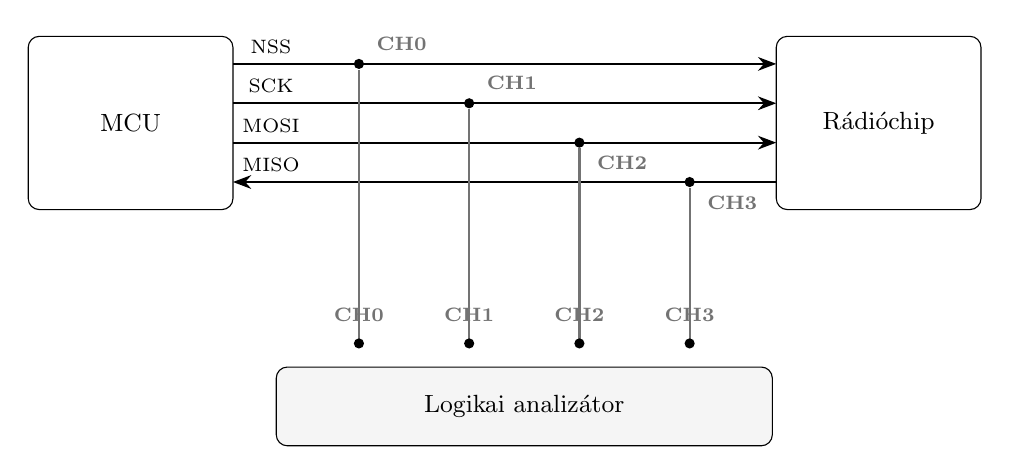
\begin{tikzpicture}[
  chip/.style={draw, rounded corners, align=center, minimum width=2.6cm, minimum height=2.2cm, font=\small},
  ana/.style={draw, rounded corners, align=center, minimum height=1.0cm, font=\small, fill=gray!8},
  sig/.style={-{Stealth}, thick},
  tap/.style={fill=black, circle, inner sep=1.3pt},
  tapline/.style={color=black!55, thick},
  chlabel/.style={font=\scriptsize\bfseries, color=black!55}
]
\node[chip] (mcu) at (0,0) {MCU};
\node[chip] (radio) at (9.5,0) {Rádióchip};
\draw[sig] (1.3,0.75) -- node[above, pos=0.07, font=\scriptsize]{NSS} (8.2,0.75);
\draw[sig] (1.3,0.25) -- node[above, pos=0.07, font=\scriptsize]{SCK} (8.2,0.25);
\draw[sig] (1.3,-0.25) -- node[above, pos=0.07, font=\scriptsize]{MOSI} (8.2,-0.25);
\draw[sig] (8.2,-0.75) -- node[above, pos=0.93, font=\scriptsize]{MISO} (1.3,-0.75);
\node[tap] (t0) at (2.9,0.75) {};
\node[tap] (t1) at (4.3,0.25) {};
\node[tap] (t2) at (5.7,-0.25) {};
\node[tap] (t3) at (7.1,-0.75) {};
\node[chlabel, anchor=south west] at (3.0,0.8) {CH0};
\node[chlabel, anchor=south west] at (4.4,0.3) {CH1};
\node[chlabel, anchor=north west] at (5.8,-0.3) {CH2};
\node[chlabel, anchor=north west] at (7.2,-0.8) {CH3};
\draw[tapline] (t0) -- (2.9,-2.8);
\draw[tapline] (t1) -- (4.3,-2.8);
\draw[tapline] (t2) -- (5.7,-2.8);
\draw[tapline] (t3) -- (7.1,-2.8);
\node[ana, minimum width=6.3cm] (la) at (5.0,-3.6) {Logikai analizátor};
\foreach \x/\lbl in {2.9/CH0, 4.3/CH1, 5.7/CH2, 7.1/CH3} {
  \node[tap] at (\x,-2.8) {};
  \node[chlabel, anchor=south] at (\x,-2.65) {\lbl};
}
\end{tikzpicture}}
\caption{Az MCU--rádióchip SPI-busz pin-kiosztása és a logikai analizátor
csatornáinak hozzárendelése (CH0=NSS, CH1=SCK, CH2=MOSI, CH3=MISO) --
minden csatorna egyenes, kereszteződésmentes vonallal a saját jeléhez kötve.}
\end{figure}

Az SPI-protokoll paraméterei: CPOL=0, CPHA=0, MSB first, CS active low.
A szükséges mintavételi frekvencia a rádióchip SPI-sebességének legalább
kétszerese (jellemzően $\geq$20~MHz).

\subsection{FIFO-írás detekció}

A rádióchip SPI-kommunikáció első bájtja kódolja a műveletet:
\begin{itemize}
    \item $\text{byte} \mathbin\& 0\text{x}80 = 0\text{x}80$: írás
    \item $\text{byte} \mathbin\& 0\text{x}7\text{F}$: regisztercím
\end{itemize}

A RegFifo (0x00) írása (\texttt{0x80}-as első bájt) tartalmazza a
LoRaWAN keretet. Tipikus TX-sorozat:
\needspace{6cm}
\begin{lstlisting}[language={},caption={SPI TX sorozat -- Join Request adás előtt}]
NSS low  0x8D 0x80  NSS high   ; FifoTxBaseAddr = 0x80
NSS low  0x8E 0x80  NSS high   ; FifoAddrPtr = 0x80
NSS low  0x80 [23 bytes]        ; FIFO write  <- LoRaWAN keret itt
NSS low  0xA2 0x17  NSS high   ; PayloadLength = 23
NSS low  0x81 0x83  NSS high   ; OpMode = TX
\end{lstlisting}

\subsection{Eredmények}

A FIFO-írás sikeresen detektálható volt, a teljes Join~Request keret
kiolvasható volt:

\needspace{7cm}
\begin{lstlisting}[caption={SPI-busz tap eredménye}]
FIFO WRITE #1  [tranzakcio #312]
PHY (23 B): 0024a59d8b75d4cf06cd8c89b5f4ee263a628ef9138d2f
Tipus:    Join Request
AppEUI:   06cfd4758b9da524
DevEUI:   3a26eef4b5898ccd
DevNonce: 8e62
MIC:      f9138d2f
\end{lstlisting}

A kinyert AppEUI és DevEUI megegyezett a szerveren regisztrált értékekkel,
megerősítve a támadás sikerét. Firmware-szintű titkosítás bekapcsolt állapota esetén
a flash-dump plaintext kulcsot nem ad vissza, de az SPI-tap a futásidejű
adatot rögzíti, így ez a védelmi intézkedés az SPI-tap fenyegetésével szemben
csak részleges.

A mérést egy 20~MHz-es mintavételi frekvenciájú, 33\,554\,432 mintás
(kb.\ 1{,}68~másodperces) capture-ablakon végeztük, amely 571 SPI-tranzakciót
tartalmazott; ebből egyetlen tranzakció volt FIFO-írás (a fenti Join~Request),
ami megfelel az elvárt viselkedésnek -- a rádióchip csak adás előtt írja a
FIFO-t, a többi tranzakció regiszter-konfiguráció és állapotlekérdezés.

\paragraph{Megjegyzés a chip-lefedettségről.} Az eszköz-oldali kinyerő
implementáció a vizsgált SX1276-alapú (V2) rádiómodulon túl előkészítve
tartalmazza az SX1262-alapú (V3/V4) csomópontok támogatását is (más
FIFO-írás parancskódolással). Ez az út egységteszteken és szintetikus,
kézzel összeállított Join~Request mintán helyesen működik, de -- mivel nem
állt rendelkezésre valódi SX1262-alapú hardveres capture -- \textbf{valós
hardveren nem lett ellenőrizve}, ezért az eredmények közé itt tudatosan nem
került be: a dolgozat kizárólag a ténylegesen hardveren igazolt SX1276/V2
méréseket közli önálló eredményként.

\subsection{A támadási felület architekturális korlátai -- integrált rádiós
(STM32WL-osztályú) eszközök}

A fenti SPI-tap támadás előfeltétele, hogy az MCU és a rádiócsip két önálló
lapka legyen, közöttük kívülről hozzáférhető SPI-busszal -- ez a vizsgált,
viszonylag olcsó Heltec-node-ok (ESP32 + külső SX1276/SX1262 rádiócsip)
esetén fennáll. A tesztkörnyezetben emellett egy jóval drágább, STM32WL55
MCU-alapú ipari fejlesztőpanel (NUCLEO-WL55JC1) is rendelkezésre állt,
amelyen a LoRa rádió a mikrokontroller lapkájába van integrálva -- nincs
önálló, kívülről hozzáférhető rádiócsip, így nincs lehallgatható külső
MCU--rádiócsip SPI-busz sem.

Ez azt jelenti, hogy a jelen fejezetben bemutatott támadási felület a
STM32WL-osztályú eszközökön architekturálisan nem létezik, függetlenül
bármilyen firmware-szintű hardeningtől -- nem egy konfigurálható védelem
szünteti meg, hanem maga a lapka-integráció zárja ki eleve. (A STM32WL-en
egyébként is azonosított, debug-port-alapú fizikai támadási felületet a
8.\ fejezet külön tárgyalja.) Ez önmagában egy dokumentálható
biztonsági-gazdasági következtetés, új mérés nélkül: az olcsóbb, kéttagú
(MCU + külső rádiócsip) node-architektúra extra fizikai támadási felületet
nyit, amit a drágább, integrált rádiós platform megválasztása önmagában,
mérés nélkül is kizár -- a SPI-tap fenyegetés szempontjából tehát a
magasabb hardverköltség közvetlenül magasabb fizikai biztonsági szintet
jelent.

% -----------------------------------------------------------------------
\section{AppKey brute-force -- Join Request MIC alapján}
% -----------------------------------------------------------------------

\subsection{Elv}

A Join~Request MIC számítása:
\begin{equation}
    \text{MIC} = \text{AES-128-CMAC}(\text{AppKey},\
    \text{MHDR} \mathbin\| \text{AppEUI} \mathbin\|
    \text{DevEUI} \mathbin\| \text{DevNonce})[0:4]
\end{equation}

Mivel a MIC inputja (MHDR, AppEUI, DevEUI, DevNonce) a levegőből
passz\-ív\-an rögzíthető (ld.\ 4.\ fejezet), egy támadó az összes AppKey-jelöltet
offline, hálózati hozzáférés nélkül tesztelheti: minden jelöltre kiszámítja
az AES-128-CMAC-ot, és összehasonlítja az utolsó 4 bájttal. Ugyanezt az elvet
nyilvános, offenzív biztonsági eszközök (pl.\ a LoraPWN és a Loracrack
projektek) is alkalmazzák gyenge/alapértelmezett AppKey-ek ellen, megerősítve,
hogy ez nem elméleti, hanem a gyakorlatban is aktívan kihasznált
támadási út~\cite{gauging2021, loracrack2025}.

\subsection{Implementáció}

Az eszköz három módot támogat:

\begin{enumerate}
    \item \textbf{Wordlist mód:} ismert gyenge/alapértelmezett kulcsok listája
    (gyártói alapértelmezések, nulla kulcs, DEADBEEF\ldots mintás kulcsok).
    \item \textbf{Szekvenciális mód:} az összes legfeljebb $N$ darab nemnulla
    bájtot tartalmazó 128 bites kulcs kimerítő keresése.
    \item \textbf{Hybrid mód:} wordlist először, majd szekvenciális keresés
    (alapértelmezés).
\end{enumerate}

A belső ciklus Python \texttt{cryptography} könyvtár AES-128-CMAC implementációját
alkalmazza; egyetlen magos futás kb.\ $10^6$ kulcsot/s sebességen tesztel.

\subsection{Eredmények}

\begin{table}[H]
\centering
\caption{AppKey brute-force teszteredmények}
\begin{tabular}{llr}
\toprule
Kulcs-típus & Mód & Időigény \\
\midrule
\texttt{00:00:\ldots:00} (nulla kulcs) & wordlist & $<1$~ms \\
Gyártói alapértelmezés & wordlist & $<50$~ms \\
Legfeljebb 1 nemnulla bájt & szekvenciális & $\approx 3$~s \\
Legfeljebb 2 nemnulla bájt & szekvenciális & $\approx 45$~perc \\
\bottomrule
\end{tabular}
\end{table}

A teszt során a nulla kulcsot és több ismert gyártói alapértelmezést sikeresen
visszaállítottunk. Erős, véletlenszerű 128 bites kulcsok esetén a brute-force
nem kivitelezhető a jelenlegi számítási kapacitással.

\begin{figure}[H]
\centering
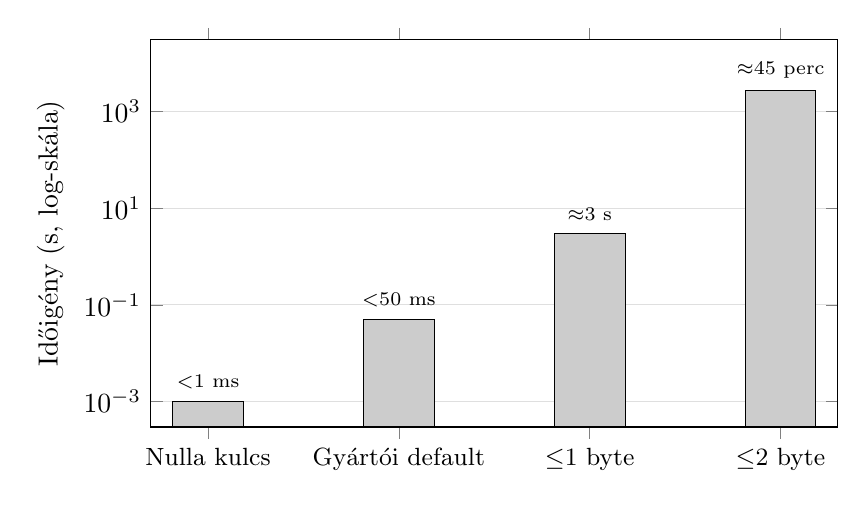
\begin{tikzpicture}
\begin{axis}[
  ybar,
  bar width=0.9cm,
  width=0.85\textwidth,
  height=6.5cm,
  ymode=log,
  log origin=infty,
  ymin=0.0003, ymax=30000,
  ylabel={Időigény (s, log-skála)},
  symbolic x coords={Nulla kulcs,Gyártói default,$\leq$1 byte,$\leq$2 byte},
  xtick=data,
  x tick label style={font=\small, align=center},
  ymajorgrids, major grid style={gray!25},
]
\addplot[fill=gray!40, draw=black] coordinates {
  (Nulla kulcs,0.001)
  (Gyártói default,0.05)
  ($\leq$1 byte,3)
  ($\leq$2 byte,2700)
};
\node[font=\scriptsize, anchor=south] at (axis cs:Nulla kulcs,0.001) [yshift=1pt] {$<$1 ms};
\node[font=\scriptsize, anchor=south] at (axis cs:Gyártói default,0.05) [yshift=1pt] {$<$50 ms};
\node[font=\scriptsize, anchor=south] at (axis cs:$\leq$1 byte,3) [yshift=1pt] {$\approx$3 s};
\node[font=\scriptsize, anchor=south] at (axis cs:$\leq$2 byte,2700) [yshift=1pt] {$\approx$45 perc};
\end{axis}
\end{tikzpicture}
\caption{Az AppKey brute-force időigénye kulcstípusonként (log-skála; a
mért értékek az előző táblázattal egyeznek).}
\end{figure}

\subsection{A teljes lánc hardveren, kulcs nélküli RF-outsiderként validálva}

A fenti offline crackert egy teljes, kulcs nélküli RF-outsider forgatókönyvben
is végigvittük: a támadó kizárólag a levegőből fogott adatokkal dolgozik,
sem hálózati (API/MQTT), sem fizikai (SPI/debug-port) hozzáférése nincs az
áldozathoz.

Az áldozat egy Heltec~V3 panel, szándékosan gyenge, a gyakorlatban széles
körben elterjedt tutorial-kulccsal
(\texttt{0102030405060708090A0B0C0D0E0F10}) felprogramozva, amely bootolás
után folyamatosan OTAA Join~Requestet küld. A független RF-támadói
eszköz egy második panel (Heltec~V4), amely saját rádiójával, nyers
LoRa-vételi módban, a Join-csatornán (868,1~MHz, SF9, BW125) figyel -- ez
a csatorna/SF-pár egy korábbi, egyszeri instrumentált megfigyelésből derült
ki, a tényleges crack-láncban már nincs rá szükség. A V4 kilenc Join~Requestet
fogott el a levegőből (RSSI~$\approx-120$~dBm, tehát valódi, gyenge RF-vétel,
nem vezetékes lehallgatás), növekvő DevNonce-értékekkel.

A \texttt{appkey\_crack.py} eszköz mind a kilenc, kizárólag RF-en elfogott
kereten ugyanarra a gyenge kulcsra tört -- a crack-lépés tehát bizonyítottan
nem igényel semmilyen, az RF-vételen túli információt. Kontrollként egy
valódi, véletlenszerű 128 bites kulccsal felprogramozott eszközön (ld.\
fent, a keylessoutsider-sweep részeként, 9.\ fejezet) ugyanez a lépés
elbukik -- a támadás tehát bizonyítottan gyengekulcs-specifikus, nem a
LoRaWAN Join-eljárás vagy a MIC-séma hibája.

A \emph{weaponizálás} lépésben a feltört kulcsot a hálózati szerverbe is
regisztráltuk, és egy újabb, valódi Join-cserét figyeltünk meg. A
sniffelt+feltört anyagból (titkosított Join~Accept, DevNonce) levezetett
NwkSKey és AppSKey \textbf{bitre megegyezett} a hálózati szerver belső
munkamenet-állapotával. A levezetett AppSKey-jel egy valódi, az áldozat
által később küldött titkosított uplink FRMPayload-ját is sikeresen
visszafejtettük, az eredeti (\texttt{0xA5}) payload-értéket helyreállítva --
ez a bizalmasság teljes körű megtörését demonstrálja, a NwkSKey birtokában
pedig a keret-hamisítás lehetősége is adott.

\textbf{Severity-keretezés:} ez a lánc a célpont kulcskezelési hibáját
(gyenge/alapértelmezett AppKey) aknázza ki, nem a LoRaWAN-protokoll vagy a
ChirpStack kriptográfiájának hibáját -- rendes, véletlenszerű AppKey esetén
a lánc már a crack-lépésnél elbukik. A teljes lánc (RF-sniff $\to$ offline
crack $\to$ munkamenetkulcs-levezetés $\to$ forgalom visszafejtése) valódi
hardveren és valós kriptográfiai műveletekkel igazolt, 2026-10-05-én.

% -----------------------------------------------------------------------
\section{Firmware-bináris elemzés és álcázott csomópont}
% -----------------------------------------------------------------------

\subsection{Elv}

A firmware-bináris az AppKey-t, DevEUI-t és AppEUI-t statikusan tárolja.
Ha az eszközhöz fizikai hozzáféréssel rendelkezünk, a flash tartalmát
a gyártó által biztosított eszközzel kiolvashatjuk (pl.\ bootloader módban).
Firmware-szintű titkosítás nélkül a bináris plaintext; titkosítással védett
esetén a debug interfészen keresztül olvasható, ha az nincs letiltva.

\subsection{Kulcskinyerés a binárisból}

Az eszköz két stratégiát alkalmaz:

\begin{enumerate}
    \item \textbf{Közvetlen kulcskeresés (Strategy A):} az ismert AppKey
    bájt-mintájának mindkét bájt-sorrendben (LE/BE) keresése a binárisban.
    A firmware stack kulcstárolási elrendezésétől függően a DevEUI és AppEUI
    a megtalált kulcs közelében helyezkednek el.

    \item \textbf{Entrópiaszkennelés (Strategy B):} a firmware binárisban
    szomszédos, magas entrópiájú 16 bájtos blokkok azonosítása.
    Gyártófüggetlen, különböző firmware stackeken is alkalmazható.
\end{enumerate}

\subsection{Álcázott csomópont generálása}

A kinyert hitelesítő adatok (AppKey, DevEUI, AppEUI) alapján az eszköz
automatikusan generál egy kész csomópont firmware-t (sablonból), amely:
\begin{itemize}
    \item OTAA csatlakozást hajt végre az eredeti eszköz adataival,
    \item az áldozat payload-formátumát utánzó valósághű adatokat küld,
    \item opcionálisan WiFi+MQTT C2-csatornán keresztül futásidőben
    parancsokkal irányítható.
\end{itemize}

\subsection{Eredmények és hatásvizsgálat}

A generált rogue csomópont sikeresen regisztrált a ChirpStack hálózati
szerveren az áldozat DevEUI alatt. A hálózati szerver naplójában az
álcsomópont uplink csomagjai megkülönböztethetetlenek voltak az eredeti
eszköz csomagjaitól. Az egyetlen detekciós lehetőséget a DevNonce
visszajátszás-védelem nyújtotta, azonban ha az eredeti eszköz ki van
kapcsolva, az álcsomópont zavartalan kommunikációt folytathat.

\subsection{Munkamenetkulcs-levezetés érvényesítése éles teszttel}

A fenti forgatókönyvet (fizikai hozzáféréssel korábban megszerzett AppKey
felhasználása rogue csomópont klónozására) a hálózati oldalon is
végigvittük: egy szabad fejlesztői panelt az áldozat eszköz valódi
DevEUI/AppEUI/AppKey hármasával programoztunk, majd valódi OTAA
Join-folyamatot hajtottunk végre a hálózati szerver ellen. A titkosított
Join~Accept választ -- a valós RF- vagy SPI-elfogás gyakorlati
helyettesítőjeként -- a hálózati szerver saját, adminisztratív
keretfolyam-API-ján keresztül rögzítettük, majd a levont munkamenetkulcsokat
(NwkSKey, AppSKey) a klónozott eszköz saját AppKey-jéből, a Join~Accept
titkosított tartalmából és a DevNonce-ból vezettük le, a
2.\ fejezetben leírt képlet szerint.

A levezetés helyességének ellenőrzésére a legerősebb rendelkezésre álló
próbát alkalmaztuk: a klónozott eszköz a soros konzoljára kiírta a saját,
tőlünk teljesen független firmware-implementációja által kiszámolt
DevAddr-t, amely \textbf{bit-pontosan megegyezett} az általunk, külső
eszközből levezetett DevAddr-rel. Emellett a levezetett AppSKey-jel egy
kontrollált titkosítás/visszafejtés kör (ismert plaintext $\to$
FRMPayload-titkosítás $\to$ visszafejtés) is helyesen adta vissza az
eredeti adatot, megerősítve, hogy a payload-titkosítási lánc is helyesen
lett reprodukálva.

Ez a teszt gyakorlatilag igazolja, hogy egy SPI-tappal vagy firmware-dumppal
megszerzett AppKey birtokában a támadó -- pusztán a hálózat felől
megfigyelhető (vagy elfogható) Join-forgalom alapján -- helyesen tudja
reprodukálni mindkét munkamenetkulcsot, azaz a fenti álcázott csomópont
nemcsak regisztrálni, hanem a titkosított adatforgalmat is hitelesen
generálni/értelmezni képes.

% -----------------------------------------------------------------------
\section{Védelmi mechanizmusok értékelése}
% -----------------------------------------------------------------------

\subsection{Firmware-szintű titkosítás}

A firmware-szintű titkosítás bekapcsolása után az eszköz flash-tartalma
titkosítva tárolódik; a titkosítási kulcs hardveresen védett és szoftveresen
nem olvasható. Ennek következtében:
\begin{itemize}
    \item \textbf{Hatékony:} közvetlen flash-dump (bootloader mód)
    plaintext kulcsot nem ad vissza.
    \item \textbf{Nem elégséges önmagában:} a futásidejű memória nem titkosított,
    az SPI-busz tap a Join~Request plaintext keretét rögzíti,
    és ha a debug interfész nincs letiltva, azon keresztül a RAM kiolvasható.
    Az itt használt ESP32-platformon korábban már dokumentáltak is voltak
    olyan megvalósítási hibák (pl.\ CVE-2020-15048), amelyek a flash-titkosítást
    teljes egészében megkerülhetővé tették -- ez is azt mutatja, hogy a
    védelem erőssége nem csak a bekapcsolt állapoton, hanem a konkrét
    implementáció helyességén is múlik~\cite{BV2020}.
\end{itemize}

\subsection{Biztonságos indítás (Secure Boot)}

A biztonságos indítás biztosítja, hogy csak aláírt firmware futhasson az eszközön,
a gyártói referencia-implementáció szerint~\cite{secure2026}.
Ez megakadályozza a módosított/rogue firmware feltöltését, de önmagában nem
véd a kulcskinyerés ellen, ha az eszköz fut. Hasonlóan a flash-titkosításhoz,
a secure boot implementációja is hordozhat megkerülhető hibákat -- ugyanezen
a platformcsaládon korábban nyilvánosan dokumentált hiba (pl.\
CVE-2020-13629) tette lehetővé az aláírás-ellenőrzés megkerülését
alkalmas firmware-képpel~\cite{BV2020a}.

\subsection{Megerősített firmware-konfiguráció}

Az általunk fejlesztett megerősített konfiguráció -- a biztonságos
LoRaWAN-végpontokra vonatkozó szakirodalmi ajánlásokkal
összhangban~\cite{oniga2017} -- az alábbi
intézkedéseket foglalja magában:
\begin{itemize}
    \item firmware-szintű titkosítás + biztonságos indítás egyidejű bekapcsolása,
    \item debug interfész letiltása,
    \item erős, véletlenszerű 128 bites AppKey generálása provisioning során,
    \item DevNonce-kezelés: minden Join~Request egyedi nonce, visszajátszásvédelem,
    \item alkalmazásszintű payload-titkosítás érzékeny szenzorértékekhez.
\end{itemize}

\subsection{A debug-port lezárása olvasásvédelemmel (RDP) -- hardveres igazolás}

A fenti intézkedések közül a \emph{debug interfész letiltását} valódi
hardveren, a tesztkörnyezet ipari referencia-csomópontján
(STM32WL55JC1) külön is igazoltuk, mivel ez zárja le közvetlenül a
7.\ fejezetben bemutatott firmware-kinyerési utat (a nyitott
hibakeresési porton keresztüli flash- és memória-olvasást).

\paragraph{Kiindulás (RDP Level~0).} Gyári állapotban az eszköz
olvasásvédelme kikapcsolt (az \texttt{FLASH\_OPTR} regiszter RDP-mezője
\texttt{0xAA}). Ekkor a hibakereső a teljes flash-t korlátozás nélkül
kiolvassa -- a csomópont beégetett firmware-je és abban a kulcsanyag
bitről bitre kinyerhető. Ez nem a hardver hibája, hanem \emph{hardening-elmaradás}:
a vizsgált gyári egység egyszerűen RDP~Level~0-n került forgalomba.

\paragraph{Megerősítés (RDP Level~1).} Az olvasásvédelmet Level~1-re emelve
(RDP-mező \texttt{0xBB}) a hibakereső \emph{csatlakozni} még tud, de a
védett memóriából semmit nem olvas ki: a flash és a RAM olvasása egyaránt
elutasításra kerül, sőt a mag regiszterei is kizárólag \texttt{0xFFFFFFFF}
értéket adnak vissza (a megállított magon mért programszámláló
\texttt{0xFFFFFFFE}). Lényeges, hogy a \emph{csomópont funkcionálisan
sértetlen marad}: a hardening életbe lépése után az eszköz újra
csatlakozott a hálózathoz (OTAA-join, kiosztott DevAddr, növekvő
felvételi keretszámláló) és küldte az uplinkeket -- a védelem a
kiolvasást zárja, nem a működést.

\paragraph{Visszaállíthatóság és a kulcsanyag védelme.} Az olvasásvédelem
Level~1-ről Level~0-ra csökkentése a hardver által kikényszerített
\emph{teljes flash-törlést} (mass-erase) vált ki: a művelet után a flash
minden szava \texttt{0xFFFFFFFF}. Vagyis a védett tartalom nem
visszafejthető, kizárólag megsemmisíthető -- a firmware és a benne tárolt
kulcsok így nem szivárognak ki a hibakeresési porton.

\paragraph{Következtetés.} A 7.\ fejezet firmware-kinyerési forgatókönyve
tehát \emph{egyetlen provisioning-lépéssel} (RDP~Level~1 beállítása a
gyártás végén) kivédhető, a csomópont működésének megtartása mellett. Ez
megerősíti, hogy a vizsgált eszköz kiolvashatósága nem platformszintű
sebezhetőség, hanem konfigurációs hiányosság volt. (Az RDP~Level~2
véglegesen, visszafordíthatatlanul tiltja a hibakeresést; ezt éles
eszközön ritkán indokolt alkalmazni, és a jelen munkában tudatosan nem
teszteltük.)

\paragraph{Korlát: a szoftveres olvasásvédelem feszültség-/óraglicheléssel
megkerülhető.} Fontos leszögezni, hogy az RDP~Level~1 \emph{szoftveresen}
nyújt védelmet -- más gyártók mikrokontrollerein (pl.\ STM32, Nordic nRF52)
nyilvánosan dokumentált, feszültség- vagy óra-glicheléssel (voltage/clock
glitching) kivitelezett támadások ismertek, amelyek a hasonló célú
olvasásvédelmi mechanizmusokat fizikai szinten kerülik meg, kifejezetten
ezen bitek hardveres ellenőrzésének pillanatnyi megzavarásával~\cite{Kesenheimer2025,
Secure2025, Soler2025}. Ez a jelen tesztkörnyezetben rendelkezésre álló
eszközparkkal (alacsony költségű oszcilloszkóp, logikai analizátor) nem
volt kivitelezhető, és a dolgozat keretein kívül eső, jövőbeli kutatási
iránynak minősül (ld.\ 9.\ fejezet).

\subsection{A védelmi szint összefoglalása}

\begin{table}[H]
\centering
\caption{Védelmi mechanizmusok hatékonysága a demonstrált támadásokkal szemben}
\begin{tabular}{lcccc}
\toprule
Védelmi intézkedés & Passzív & SPI-tap & Brute- & Firmware- \\
                   & sniff   &         & force  & dump \\
\midrule
(nincs)                              & -- & -- & -- & -- \\
Fw. titkosítás                       & -- & -- & -- & \checkmark \\
Fw. titkosítás + debug tiltás        & -- & -- & -- & \checkmark\checkmark \\
RDP Level~1 (olvasásvédelem)$^\dagger$ & -- & -- & -- & \checkmark\checkmark \\
Fw. titkosítás + biztonságos indítás & -- & -- & -- & \checkmark\checkmark \\
Erős AppKey                          & -- & -- & \checkmark & -- \\
\textbf{Teljes hardened konfig.}     & -- & -- & \checkmark & \checkmark\checkmark \\
\bottomrule
\multicolumn{5}{l}{\footnotesize \checkmark\ = hatékony,
\checkmark\checkmark\ = erős védekezés, --\ = nem nyújt védelmet} \\
\multicolumn{5}{l}{\footnotesize $^\dagger$ valódi hardveren igazolva
(STM32WL55JC1) -- ld.\ az előző alfejezetet}
\end{tabular}
\end{table}

\noindent Az SPI-busz tap és a passzív sniffing ellen szoftveres intézkedések
önmagukban nem nyújtanak védelmet. A fizikai biztonsági intézkedések
(tamper-evident tokozás, érintési érzékelők) szükségesek az SPI-tap
fenyegetésének hatékony kezeléséhez.

\begin{figure}[H]
\centering
\resizebox{\textwidth}{!}{%
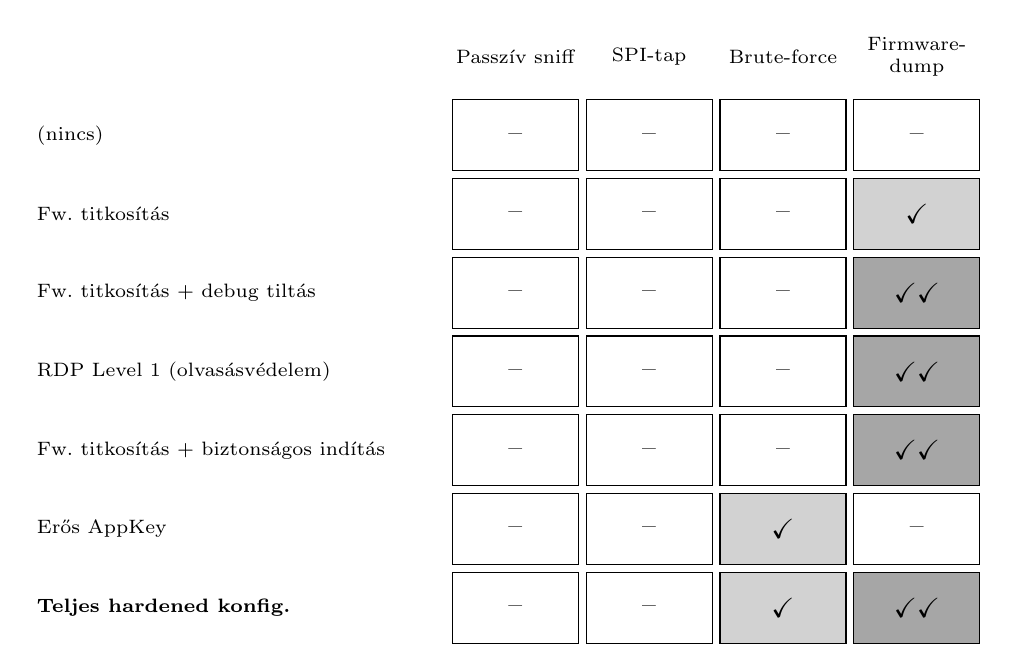
\begin{tikzpicture}[
  cell0/.style={draw, fill=white, minimum width=1.6cm, minimum height=0.9cm},
  cell1/.style={draw, fill=gray!35, minimum width=1.6cm, minimum height=0.9cm},
  cell2/.style={draw, fill=gray!70, minimum width=1.6cm, minimum height=0.9cm},
  lbl/.style={font=\scriptsize, align=left, anchor=west},
  hdr/.style={font=\scriptsize, align=center}
]
\def\cA{6.2} \def\cB{7.9} \def\cC{9.6} \def\cD{11.3}
\def\rH{0}
\def\rA{-1.0} \def\rB{-2.0} \def\rC{-3.0} \def\rD{-4.0}
\def\rE{-5.0} \def\rF{-6.0} \def\rG{-7.0}
\node[hdr, text width=1.6cm] at (\cA,\rH) {Passzív sniff};
\node[hdr, text width=1.6cm] at (\cB,\rH) {SPI-tap};
\node[hdr, text width=1.6cm] at (\cC,\rH) {Brute-force};
\node[hdr, text width=1.6cm] at (\cD,\rH) {Firmware-dump};
\node[lbl, text width=5.6cm] at (0,\rA) {(nincs)};
\node[lbl, text width=5.6cm] at (0,\rB) {Fw.\ titkosítás};
\node[lbl, text width=5.6cm] at (0,\rC) {Fw.\ titkosítás + debug tiltás};
\node[lbl, text width=5.6cm] at (0,\rD) {RDP Level~1 (olvasásvédelem)};
\node[lbl, text width=5.6cm] at (0,\rE) {Fw.\ titkosítás + biztonságos indítás};
\node[lbl, text width=5.6cm] at (0,\rF) {Erős AppKey};
\node[lbl, text width=5.6cm, font=\scriptsize\bfseries] at (0,\rG) {Teljes hardened konfig.};
\node[cell0] at (\cA,\rA) {--}; \node[cell0] at (\cB,\rA) {--};
\node[cell0] at (\cC,\rA) {--}; \node[cell0] at (\cD,\rA) {--};
\node[cell0] at (\cA,\rB) {--}; \node[cell0] at (\cB,\rB) {--};
\node[cell0] at (\cC,\rB) {--}; \node[cell1] at (\cD,\rB) {\checkmark};
\node[cell0] at (\cA,\rC) {--}; \node[cell0] at (\cB,\rC) {--};
\node[cell0] at (\cC,\rC) {--}; \node[cell2] at (\cD,\rC) {\checkmark\checkmark};
\node[cell0] at (\cA,\rD) {--}; \node[cell0] at (\cB,\rD) {--};
\node[cell0] at (\cC,\rD) {--}; \node[cell2] at (\cD,\rD) {\checkmark\checkmark};
\node[cell0] at (\cA,\rE) {--}; \node[cell0] at (\cB,\rE) {--};
\node[cell0] at (\cC,\rE) {--}; \node[cell2] at (\cD,\rE) {\checkmark\checkmark};
\node[cell0] at (\cA,\rF) {--}; \node[cell0] at (\cB,\rF) {--};
\node[cell1] at (\cC,\rF) {\checkmark}; \node[cell0] at (\cD,\rF) {--};
\node[cell0] at (\cA,\rG) {--}; \node[cell0] at (\cB,\rG) {--};
\node[cell1] at (\cC,\rG) {\checkmark}; \node[cell2] at (\cD,\rG) {\checkmark\checkmark};
\end{tikzpicture}}
\caption{A védelmi mechanizmusok hatékonysága a négy demonstrált támadással
szemben (vizuális összefoglaló az előző táblázathoz: fehér = nem nyújt
védelmet, világosszürke = hatékony, sötétszürke = erős védekezés).}
\end{figure}

\subsection{Az OTA-frissítési csatorna hardeningje}

A fenti intézkedések a végponti kulcsanyag védelmére irányulnak; a
tesztkörnyezetben emellett a hálózati szerver és a végpontok közötti
\emph{firmware-frissítési} csatorna megerősítését is elvégeztük és valódi
hardveren, éles ChirpStack-en keresztül ellenőriztük.

\paragraph{Tervezési alap.} A LoRaWAN specifikáció (sem az 1.0.x, sem az
1.1-es verzió) nem ír elő OTA-frissítési biztonsági mechanizmust -- ez
kívül esik a protokoll hatókörén, a rádiós/Join-réteget szabványosítja,
nem az alkalmazás-szintű firmware-disztribúciót. Az itt megvalósított
aláírt manifeszt + anti-rollback + integritásvédelem hármas ezért nem egy
LoRaWAN-specifikus előírást követ, hanem az IETF SUIT (Software Updates
for IoT) munkacsoport jelenleg érvényben lévő, korlátozott erőforrású IoT
eszközökre szabott architektúráját és manifeszt-információs modelljét
alkalmazza erre a rétegre: aláírt/hitelesített és integritásvédett
firmware-kép, szekvenciaszám-alapú anti-rollback-védelem, valamint a
frissítés metaadatait leíró manifesztum -- pontosan a három elv, amit a
tesztkörnyezetben implementáltunk és hardveren
igazoltunk~\cite{rfc9019, rfc9124}.

\paragraph{Aláírt manifeszt, anti-rollback, chunk-szintű integritás.} A
frissítési protokoll aláírt manifeszttel indul, majd darabolt (chunk)
adatátvitellel folytatódik, munkamenet-azonosítóval (session ID) és
chunk-szintű CRC8-cal, a teljes image SHA-256 ellenőrzésével lezárva. Egy
teljes, megszakítás nélküli, hardveres tesztfuttatásban mind a 6 adatkeret
session ID-je és CRC8-a helyesnek bizonyult, a teljes átvitel SHA-256
hash-e pontosan egyezett az aláírt manifesztben szereplő értékkel, és a
végső, natív image-validáció (chip-ID ellenőrzés) is a várt módon utasította
el a szintetikus (nem valós firmware-t tartalmazó) tesztadatot -- vagyis a
védelem minden rétege külön-külön, kimutathatóan működött.

\paragraph{Munkamenet-izolláció -- véletlenül reprodukált pozitív eset.} Egy
megszakadt, majd új munkamenettel újraindított átvitel során az eszköz
helyesen utasította el egy korábbi, már nem aktív munkamenethez tartozó
adatkeretek fogadását (\texttt{session mismatch, ignoring}) -- ez a
session-alapú izoláció tényleges, akaratlanul előidézett próbája volt,
amely megerősítette, hogy idegen/elavult átviteli kísérletek nem tudják
befolyásolni egy folyamatban lévő, más munkamenethez tartozó frissítést.

\paragraph{Kezelési csatorna: TLS + minimál jogosultságú API-kulcs.} A
frissítést vezérlő eszköz és a ChirpStack API közötti gRPC-csatorna
korábban titkosítatlan volt annak ellenére, hogy az API-kulcs gyakorlatilag
teljes hozzáférést biztosít. A vizsgált ChirpStack-verzió (v4.19.0) natív
API-oldali TLS-t nem támogat, ezért a csatornát egy reverse proxy mögé
helyeztük; a TLS-védett kapcsolatot végponttól végpontig ellenőriztük
(tanúsítványlánc-validáció, hitelesített gRPC-hívás). Emellett az eddig
használt, ideiglenes, teljes admin-jogú API-kulcsot egy állandó,
tenant-szintre korlátozott kulcsra cseréltük, amelynek működését valódi,
regisztrált eszközön is megerősítettük.

\paragraph{Mért, még nyitott korlát.} A hardveres teszt egy tényleges
megbízhatósági rést is felszínre hozott: a hálózati szerver a downlink
\emph{kiküldését} (queue kiürülését) jelzi sikeresként, nem az eszköz
tényleges \emph{vételét} -- egy mérésben a szerver 6/6 chunk sikeres
kézbesítését jelezte, miközben az eszköz naplója szerint csak 4 érkezett
meg ténylegesen. Ez konkrét, mért bizonyíték arra, hogy megbízható OTA-hoz
nyugtázott (confirmed) downlink vagy alkalmazásszintű ACK szükséges --
ez jelenleg nincs bevezetve, a 9.\ fejezet jövőbeli irányai között
szerepel.

% -----------------------------------------------------------------------
\section{Összefoglalás és jövőbeli kutatási irányok}
% -----------------------------------------------------------------------

\subsection{Összefoglalás}

Jelen dolgozatban négy LoRaWAN-specifikus támadási forgatókönyvet valósítottunk
meg és értékeltünk egy kontrollált tesztkörnyezetben:

\begin{enumerate}
    \item \textbf{Passzív SDR sniffing:} a Join~Request teljes metaadatkészlete
    (AppEUI, DevEUI, DevNonce, MIC) hálózati hozzáférés nélkül rögzíthető
    olcsó, kereskedelemben elérhető eszközzel.

    \item \textbf{SPI-busz tap:} fizikai hozzáféréssel a LoRaWAN keret az adás
    előtt plaintext formában kiolvasható a rádióchip FIFO-írásából, firmware-szintű
    titkosítás bekapcsolt állapotában is.

    \item \textbf{AppKey brute-force:} gyenge vagy alapértelmezett kulcsok esetén
    a rögzített Join~Request MIC alapján az AppKey másodpercek-percek alatt
    helyreállítható offline brute-force-szal.

    \item \textbf{Firmware-elemzés és rogue csomópont:} flash-dumpból az AppKey,
    DevEUI és AppEUI automatizáltan kinyerhető; a generált álcsomópont
    megkülönböztethetetlenül kommunikál a hálózattal az eredeti eszköz identitásával.
\end{enumerate}

Az eredmények megerősítik, hogy a LoRaWAN kriptográfiai védelme erős, de
a fizikai eszközbiztonság és a kulcsmenedzsment gyengeségei szignifikáns
kockázatot jelentenek a valós telepítésekben.

\subsection{Kiegészítő eredmények: hálózatszerver- és keretszintű vizsgálatok}

A fő négy forgatókönyv mellett három, opportunista jellegű kiegészítő
vizsgálatot is lezártunk, amelyek nem a LoRaWAN-protokollt, hanem a
hálózati szerver (ChirpStack) és a kulcs nélküli RF-felület határait
térképezik fel.

\textbf{ChirpStack eszközprofil-kódek, erőforrás-kimerítés:} egy
payload-vezérelt, szándékosan végtelen ciklust tartalmazó kódek-script
nem okozott erőforrás-kimerítési (DoS) hatást a hálózati szerveren -- a
vizsgált ChirpStack~4.19.0 a kódek-futásidőt korlátozza, időtúllépés
esetén a dekódolt objektum \texttt{null} lesz, a szerver válaszképes
marad. Negatív eredmény, de a korlátozás hiányában a kockázat valós
lenne.

\textbf{Kódek-injekció a nyelőig:} ugyanazon kódek-rétegen keresztül egy
célzottan összeállított on-wire string sanitizálatlanul, verbátim eljut
egy MQTT-integráción át egy mintaszerű üzemeltetői webes irányítópultig.
Egy \texttt{innerHTML}-alapú DOM-nyelőn keresztül ez markup-injekcióhoz,
weaponizált payloaddal pedig script-végrehajtáshoz vezet az üzemeltető
böngésző-originjében (tárolt XSS); \texttt{textContent} használata a
nyelőnél megszünteti a sebezhetőséget. A hiba súlyossága alkalmazásrétegi
(saját kódek és irányítópult-implementáció), nem a ChirpStack magjáé.

\textbf{Kulcs nélküli RF-outsider sweep:} egy rendesen, véletlenszerű
AppKey-jel kulcsolt eszköz esetén egy kulcs nélküli, csak RF-hozzáféréssel
rendelkező támadó nem tud kulcsot vagy munkamenetadatot kinyerni (ld.\ a
6.\ fejezet negatív kontrollja). Egyetlen, alacsony súlyosságú találat
maradt: a hálózati szerver nem korlátozza a Join~Request-ek rátáját,
ezáltal egy folytonos, véletlen azonosítójú Join-flood elérhetőségi
(availability) kockázatot jelenthet, hitelesítés vagy emberi beavatkozás
nélkül. Két további, csomagformátum-határt feszegető variáns (minimális
hosszúságú és csonkított MIC-ű keret) tiszta negatív eredményt adott --
a vizsgált LoRaWAN-keretelemző robusztusan kezelte ezeket.

\subsection{Jövőbeli kutatási irányok}

\begin{itemize}
    \item \textbf{Nyugtázott (confirmed) OTA-downlink bevezetése:} a mért
    hamis-pozitív kézbesítési jelzés (ld.\ 8.5.\ alfejezet) kiküszöbölése
    confirmed downlinkkel vagy alkalmazásszintű ACK-kal.
    \item \textbf{OTA integrált rádiós (STM32WL-osztályú) csomóponton:} a
    mérések szerint a vizsgált integrált MCU+rádió eszköz 256~KB-os,
    egybankos belső flash-e nem elegendő a teljes-image (A/B) OTA-hoz --
    a futó és a staging-image együtt nem fér el, és nincs hardveres
    bank-váltás az aktiváláshoz. Ennek feloldása külső SPI-flash alapú
    staging + saját másodlagos bootloader, vagy a gyártói biztonságos
    frissítési keret (ST SBSFU) bevonása; ez a rész önálló tervezési
    és megvalósítási feladat.
    \item \textbf{LoRaWAN~1.1 biztonsági értékelése:} a DevNonce-kezelés és
    a JoinEUI mechanizmus vizsgálata a LoRaWAN~1.1-es specifikáció alapján.
    \item \textbf{Bit-flipping és MIC-hamisítás:} NwkSKey nélküli csomagmódosítás
    határainak vizsgálata érzékeny ipari alkalmazásokban.
    \item \textbf{Hálózati szintű anomáliadetekcó:} gépi tanulás alapú
    rendellenesség-detekció megvalósítása ChirpStack platformon a rogue csomópont
    detekciójára.
    \item \textbf{Több eszközcsalád vizsgálata:} a megvalósított eszközkészlet
    kiterjesztése más LoRaWAN-eszközökre (RAK4631, TTGO T-Beam, Seeed LoRa-E5).
    \item \textbf{Tamper-védelem hatékonysága:} fizikai tamper-érzékelők
    (accelerometer-alapú, fénydetektor) integrálásának vizsgálata az SPI-tap ellen.
    \item \textbf{Feszültség-/óraglicheléses eszközbeszerzés:} a 8.\ fejezetben
    említett, más gyártói platformokon dokumentált glitching-alapú RDP-megkerülés
    (\cite{Kesenheimer2025, Secure2025, Soler2025}) tényleges kipróbálása a
    STM32WL-en, dedikált glitch-hardver (pl.\ ChipWhisperer-Nano/Husky,
    PicoGlitcher) beszerzése esetén.
    \item \textbf{Hálózati szerver háttérrendszerek nagyléptékű biztonsági
    felmérése:} a jelen dolgozat egyetlen, kontrollált ChirpStack-példányra
    fókuszál; nagyszámú, éles IoT-háttérrendszer (MQTT/CoAP/XMPP-alapú)
    biztonsági állapotát vizsgáló nagyléptékű mérések rámutatnak, hogy az
    itt talált konfigurációs hiányosságok (pl.\ gyenge AppKey, hiányzó
    rate-limit) iparági léptékben is tipikusak~\cite{Tagliaro2024}.
    \item \textbf{Automatizált LoRaWAN biztonsági tesztelő keretrendszer:} a
    jelen munkamenetben kézzel összeállított PoC-ok helyett egy dedikált,
    újrafelhasználható tesztelő keretrendszer (pl.\ a ChirpOTLE mintájára)
    bevezetése rendszeresebb regressziós biztonsági teszteléshez~\cite{Hessel2020}.
\end{itemize}

% -----------------------------------------------------------------------
\newpage
\bibliographystyle{unsrt}
\bibliography{manual_refs,zotero_refs}
% -----------------------------------------------------------------------

\end{document}
